% Artigo científico do PHVD-APS (INF99003), formato IEEE de conferência em português.
% Compilar nesta pasta: pdflatex artigo && bibtex artigo && pdflatex artigo && pdflatex artigo
\documentclass[conference,a4paper]{IEEEtran}

\usepackage[T1]{fontenc}
\usepackage[utf8]{inputenc}
\usepackage[brazilian]{babel}
\usepackage{cite}
\usepackage{amsmath,amssymb}
\usepackage{graphicx}
\usepackage{booktabs}
\usepackage{multirow}
\usepackage{array}
\usepackage{algorithm}
\usepackage[noend]{algpseudocode}
\usepackage{xcolor}
\usepackage{tikz}
\usetikzlibrary{positioning,arrows.meta}
\usepackage{pgfplots}
\pgfplotsset{compat=1.17}
\usepackage[hidelinks]{hyperref}

\graphicspath{{../figuras/}}

\renewcommand{\IEEEkeywordsname}{Palavras-chave}
\floatname{algorithm}{Algoritmo}
\algrenewcommand\algorithmicrequire{\textbf{Entrada:}}
\algrenewcommand\algorithmicensure{\textbf{Saída:}}
\algrenewcommand\algorithmicif{\textbf{se}}
\algrenewcommand\algorithmicthen{\textbf{então}}
\algrenewcommand\algorithmicfor{\textbf{para}}
\algrenewcommand\algorithmicdo{\textbf{faça}}
\algrenewcommand\algorithmicwhile{\textbf{enquanto}}
\algrenewcommand\algorithmicreturn{\textbf{devolva}}
\algrenewcommand\algorithmicfunction{\textbf{função}}
\algrenewcommand\algorithmicrepeat{\textbf{repita}}
\algrenewcommand\algorithmicuntil{\textbf{até}}

\newcommand{\pp}{\,p.p.}

\begin{document}

\title{Planejamento mensal de visitas domiciliares a pé na Atenção Primária à Saúde: busca local com prioridade clínica, restrições operacionais e replanejamento}

\author{\IEEEauthorblockN{Gabriel P. Knopp, Matheus M. Cezar e Thiago N. da Fontoura}
\IEEEauthorblockA{Instituto de Informática, Universidade Federal do Rio Grande do Sul (UFRGS)\\
Porto Alegre, RS, Brasil}}

\maketitle

\begin{abstract}
Equipes da Atenção Primária à Saúde (APS) planejam à mão as visitas domiciliares de um território: quem visitar, em que dia, por qual equipe e em que ordem, a pé, sob jornada limitada e prazos clínicos distintos. Este trabalho formula o problema como um roteamento periódico com seleção de visitas, prazos ponderados por prioridade clínica e restrições operacionais levantadas com agentes de saúde (prazo rígido, categorias e número de profissionais, vínculo com equipe, ausências e áreas de risco), e propõe uma heurística de busca local mensal que realoca e troca visitas entre dias e equipes sob orçamento de caminhada, seguida de 1.5-opt e de um verificador formal. A heurística foi implementada num artefato aberto com roteador de caminhada próprio sobre o OpenStreetMap e avaliada em três estudos com pacientes sintéticos sobre territórios reais de Porto Alegre. Em 131 territórios, atendeu a tempo 34,63\% dos pontos de prioridade clínica, contra 28,18\% do vizinho mais próximo e 17,93\% de uma regra por urgência, com distância 1,1\% menor que a do vizinho; numa grade fatorial de 324 cenários, venceu o vizinho em 899 de 972 pares; com 250 pacientes, concluiu as visitas 5,6 dias úteis antes e com 13\% menos caminhada. Em 900 planos aleatórios com restrições combinadas, nenhuma regra foi violada.
\end{abstract}

\renewcommand{\abstractname}{Abstract}
\begin{abstract}
Primary health care teams plan home visits by hand: whom to visit, on which day, by which team and in which order, on foot, under limited shifts and distinct clinical deadlines. We model the task as periodic routing with visit selection, priority-weighted deadlines and operational constraints gathered from community health workers (hard deadlines, required professions and staff, team assignment, patient absences and risk areas), and propose a monthly local search that relocates and swaps visits across days and teams under a walking budget, followed by 1.5-opt and a formal plan verifier. The method was implemented in an open artifact with a built-in OpenStreetMap walking router and evaluated in three studies with synthetic patients on real territories of Porto Alegre, Brazil. Across 131 territories it served on time 34.63\% of clinical priority points, versus 28.18\% for nearest neighbor and 17.93\% for an urgency rule, while walking 1.1\% less than nearest neighbor; it beat nearest neighbor in 899 of 972 factorial pairs and finished a 250-patient backlog 5.6 working days earlier with 13\% less walking. No rule was violated in 900 random constrained plans.
\end{abstract}

\begin{IEEEkeywords}
visitas domiciliares, atenção primária à saúde, roteamento de veículos, busca local, replanejamento, OpenStreetMap
\end{IEEEkeywords}

\section{Introdução}

A Estratégia Saúde da Família organiza equipes multiprofissionais responsáveis por populações adscritas em territórios definidos~\cite{pnab2017,faria2020}. A visita domiciliar é uma de suas ações centrais: alcança quem não consegue ir à unidade e sustenta o acompanhamento periódico de condições crônicas~\cite{conass2021}. Na prática, a agenda dessas visitas costuma ser montada sem apoio computacional. A falta de sistemas que acompanhem pendências e intervalos entre visitas é uma fragilidade conhecida da APS~\cite{rodrigues2014}, e a adoção de tecnologia da informação nas unidades brasileiras é desigual~\cite{bender2021,pinto2024}.

O planejamento combina quatro decisões interdependentes: selecionar as visitas, escolher o dia, atribuir a equipe e ordenar as casas de cada rota a pé. A decisão de hoje muda a carga e os prazos dos dias seguintes, e faltas reais exigem replanejamento que preserve o histórico. A literatura de roteamento trata partes desse problema~\cite{toth2014,campbell2014,fikar2017}, mas o contexto da APS acrescenta prazos por condição clínica, restrições de composição de equipe e um território oficial que nem sempre coincide com quem a unidade atende.

Este trabalho investiga a seguinte questão: \emph{em instâncias representativas de visitas domiciliares com falhas de atendimento, quanto uma busca local sobre o horizonte mensal melhora o atendimento a tempo da prioridade clínica, o atraso e o deslocamento em relação a regras simples de planejamento?} A hipótese é que realocar visitas entre dias e equipes, sob um orçamento de caminhada, aumenta a prioridade atendida a tempo sem elevar o deslocamento.

As contribuições são:
\begin{enumerate}
  \item uma formulação do planejamento mensal de visitas domiciliares a pé com seleção de visitas, prazos ponderados e restrições operacionais levantadas com agentes de saúde (Seção~\ref{sec:problema});
  \item uma heurística de busca local em duas fases, com garantia gulosa de prazos rígidos, melhoria intra-rota 1.5-opt e verificação formal de todo plano (Seção~\ref{sec:metodo});
  \item um artefato aberto e instalável sem infraestrutura externa, com roteador de caminhada próprio sobre o OpenStreetMap, replanejamento após faltas e importação do cadastro da unidade (Seção~\ref{sec:artefato});
  \item uma avaliação reproduzível em três estudos sobre territórios reais, com 393, 972 e 9 comparações pareadas, além de testes de propriedade e de mutação (Seções~\ref{sec:desenho} e~\ref{sec:resultados}).
\end{enumerate}

O trabalho segue a abordagem de ciência do design~\cite{hevner2004}: o artefato é construído a partir de um problema real e avaliado experimentalmente.

\section{Trabalhos relacionados}\label{sec:relacionados}

\textbf{Roteamento de veículos.} O problema de roteamento de veículos (VRP)~\cite{dantzig1959} e suas variantes~\cite{toth2014} são a base formal do problema. Duas variantes são próximas: o VRP periódico, em que cada cliente deve ser visitado com uma frequência ao longo de um horizonte~\cite{campbell2014}, e os problemas com seleção e lucro, como o problema de orientação~\cite{vansteenwegen2011}, em que nem toda visita cabe e o objetivo pondera o que se atende. O caso aqui combina as duas: há mais demanda do que jornada, e cada visita tem prazo e peso clínico.

\textbf{Atenção domiciliar.} Revisões sobre roteamento e escalonamento em atenção domiciliar~\cite{fikar2017,cisse2017} descrevem restrições de qualificação dos profissionais, janelas de tempo e continuidade do cuidado, em geral para enfermagem domiciliar com veículos. O cenário da APS brasileira difere pelo deslocamento a pé dentro de um território adscrito, pela recorrência por condição e pela composição multiprofissional da equipe que sai junta.

\textbf{Roteamento dinâmico.} Quando informações chegam durante a execução, o plano é refeito em horizonte rolante~\cite{pillac2013}. Aqui, o evento é o resultado de cada visita: uma falta devolve a visita à fila com o prazo original.

\textbf{Saúde comunitária e OpenStreetMap.} Randriamihaja et al.~\cite{randriamihaja2024} combinam mapeamento no OpenStreetMap~\cite{haklay2008} e otimização de rotas com restrição de jornada para agentes comunitários em Madagáscar, e mostram que distâncias euclidianas subestimam os trajetos reais. Este trabalho também usa a rede de caminhada do OpenStreetMap, mas acrescenta replanejamento após eventos reais, versões do plano, comparação entre métodos e restrições levantadas com os próprios agentes.

\section{Problema}\label{sec:problema}

\subsection{Entradas}

Uma unidade de saúde (nó~0) atende pacientes $P$ dentro de um território dado por polígonos. Cada paciente $p$ tem localização e condições $C_p$; a condição $c$ tem última visita $\ell_c$ (ou um primeiro prazo), intervalo máximo $I_c$ e peso clínico $w_c \in \{1,\dots,5\}$, com prazo $d_c = \ell_c + I_c$. A janela de planejamento tem $N$ dias úteis $t_1 < \dots < t_N$ e antecipação máxima $A$. Cada equipe $k \in K$ tem jornada diária $T_k$ minutos, dias disponíveis, categorias profissionais e número de profissionais por categoria. Uma matriz possivelmente assimétrica fornece tempo $\tau_{ij}$ e distância $\delta_{ij}$ a pé entre os nós.

\subsection{Demanda}

Cada paciente gera no máximo uma visita candidata $v$ na janela, associada à condição de prazo mais próximo; $d_v$ e $w_v$ são o prazo e o peso dessa condição. A visita entra na demanda se já venceu, vence dentro do limite de antecipação $A$ ou tem prazo rígido. Seu tempo de serviço $s_v$ é a duração do atendimento mais a folga posterior, com precedência: ajuste só da próxima visita, valor próprio do paciente, folga geral do cenário.

\subsection{Decisão e restrições}

Uma solução atribui cada candidata $v$ a no máximo uma rota $r_{k,t}$ (equipe $k$, dia $t$) numa posição, ou a deixa pendente com um motivo. Cada rota começa e termina no nó~0 e satisfaz:
\begin{itemize}
  \item \emph{jornada}: $\sum_{(i,j)\in r} \tau_{ij} + \sum_{v\in r} s_v \le T_k$;
  \item \emph{compatibilidade}: $k$ tem todas as categorias exigidas por $v$, ao menos a quantidade exigida de cada uma e o número total de profissionais exigido, e é a equipe vinculada a $v$, se houver;
  \item \emph{disponibilidade}: $k$ trabalha em $t$, e $t$ não está num período de ausência do paciente;
  \item \emph{prazo rígido}: se $v$ tem prazo rígido $h_v$, deve estar numa rota com $t \le h_v$; quando isso é impossível, a pendência é marcada como obrigatória e recebe o motivo;
  \item \emph{território}: só entram pacientes dentro dos polígonos, os incluídos explicitamente pela equipe e os não transferidos.
\end{itemize}

\subsection{Critérios}

Seja $t(v)$ o dia atribuído a $v$ (para pendências, $t_N$) e $W = \sum_v w_v$. Os critérios são a \emph{prioridade atendida a tempo}, o \emph{atraso controlável ponderado} e a distância percorrida:
\begin{align}
  \Phi &= \frac{100}{W} \sum_{v \text{ atendida}} w_v \, [\, t(v) \le \max(d_v, t_1) \,], \label{eq:phi}\\
  \Delta &= \sum_{v} w_v \, \max\bigl(0,\; t(v) - \max(d_v, t_1)\bigr), \label{eq:delta}\\
  D &= \textstyle\sum_{r}\sum_{(i,j)\in r} \delta_{ij}. \label{eq:dist}
\end{align}
Em~\eqref{eq:phi} e~\eqref{eq:delta}, uma visita já vencida no início conta como a tempo se feita no primeiro dia: o atraso anterior à janela não é controlável pelo plano. Os critérios competem, e o problema generaliza o VRP com capacidade (basta $N=1$ e demanda que caiba na jornada), sendo portanto NP-difícil; daí a opção por heurísticas.

\section{Método}\label{sec:metodo}

Todo plano percorre o mesmo pipeline (Fig.~\ref{fig:pipeline}): demanda, matriz de caminhada, estratégia, garantia de prazos rígidos, melhoria intra-rota e verificação. A estratégia é o único passo substituível (padrão \emph{Strategy}), o que torna as comparações justas: todas recebem a mesma demanda e a mesma matriz.

\begin{figure}[t]
\centering
\begin{tikzpicture}[node distance=2.2mm,
  etapa/.style={draw=black!60, fill=black!4, rounded corners=2pt, font=\footnotesize, text width=0.82\columnwidth, align=left, inner sep=3pt},
  seta/.style={-{Stealth[length=1.6mm]}}]
  \node[etapa] (d) {\textbf{1. Demanda:} prazos, pesos, serviço, ausências e prazo rígido por paciente};
  \node[etapa, below=of d] (m) {\textbf{2. Matriz a pé:} rede OpenStreetMap; ruas em área de risco com peso $\times 25$};
  \node[etapa, below=of m, fill=blue!8] (s) {\textbf{3. Estratégia:} urgência, vizinho mais próximo ou busca mensal};
  \node[etapa, below=of s] (h) {\textbf{4. Prazo rígido:} inserção gulosa por prazo, retirando visitas de menor peso};
  \node[etapa, below=of h] (o) {\textbf{5. 1.5-opt:} reinserção de um nó e inversão de subsegmento em cada rota};
  \node[etapa, below=of o] (v) {\textbf{6. Verificação formal:} recusa o plano se alguma restrição for violada};
  \foreach \a/\b in {d/m,m/s,s/h,h/o,o/v} \draw[seta] (\a) -- (\b);
\end{tikzpicture}
\caption{Pipeline de planejamento. Só a etapa 3 muda entre os métodos comparados.}
\label{fig:pipeline}
\end{figure}

\subsection{Estratégias de referência}

\textbf{Urgência.} Para cada dia e equipe, ordena as candidatas já vencidas por uma pontuação de urgência (dias de atraso $\times 10$ + peso $\times 5$) e acrescenta cada uma ao fim da rota enquanto a jornada, contando a volta à unidade, comportar.

\textbf{Vizinho mais próximo.} Para cada dia e equipe, parte da unidade e acrescenta a candidata elegível e viável mais próxima em tempo de caminhada, até a jornada se esgotar.

\subsection{Busca mensal}

A heurística principal (Algoritmo~\ref{alg:busca}) parte do plano do vizinho mais próximo, garante os prazos rígidos e aplica duas fases de busca local sobre o mês inteiro. Cada movimento é a realocação de uma visita para outra rota (outro dia ou outra equipe) ou a troca de duas visitas entre rotas. O ganho de um movimento é
\begin{equation}
  g = \Delta\tau + \lambda \sum w_v\,\Delta a_v - \mu \sum w_v\,\Delta \pi_v,
\end{equation}
em que $\Delta\tau$ é a variação do tempo de caminhada, $a_v$ o atraso controlável da visita, $\pi_v \in\{0,1\}$ indica atendimento sem atraso e $\lambda = 12$ e $\mu = 24$ são minutos equivalentes a um ponto de prioridade atrasado um dia e a um ponto atendido prontamente. São parâmetros explícitos, não ajustados aos dados. A cada iteração, aplica-se o movimento viável de menor $g<0$, desde que o tempo e a distância totais não superem os do início da fase e que os pontos atendidos prontamente não diminuam. A primeira fase ($\mu=0$) só economiza caminhada e atraso; a segunda recupera pendências por inserção de menor custo, substitui visitas de peso menor (nunca as de prazo rígido) quando a jornada está cheia e repete a busca com $\mu=24$.

\begin{algorithm}[t]
\caption{Busca mensal}\label{alg:busca}
\footnotesize
\begin{algorithmic}[1]
\Require candidatas $V$, dias $t_1..t_N$, equipes $K$, matriz $(\tau,\delta)$
\State $S \gets$ \Call{VizinhoMaisPróximo}{$V$}
\State $S \gets$ \Call{GarantirPrazosRígidos}{$S$}
\State $S \gets$ \Call{Fase}{$S$, recuperar $=$ falso, $\mu = 0$}
\State \Return \Call{Fase}{$S$, recuperar $=$ verdadeiro, $\mu = 24$}
\Function{Fase}{$S$, recuperar, $\mu$}
  \State aplicar 1.5-opt a cada rota de $S$
  \If{recuperar} inserir pendências por menor $\Delta\tau + \lambda w_v a_v$ \EndIf
  \State $B_\tau, B_\delta, B_\pi \gets$ tempo, distância e pontos prontos de $S$
  \For{até 80 iterações}
    \State $m \gets$ realocação ou troca viável de menor $g$
    \State \hspace{1em}com $\tau(S') \le B_\tau$, $\delta(S') \le B_\delta$, $\pi(S') \ge B_\pi$
    \If{não há $m$ com $g < 0$} \textbf{pare} \EndIf
    \State aplicar $m$; 1.5-opt nas rotas alteradas
  \EndFor
  \If{recuperar}
    \State trocar visitas de peso menor por pendências de peso maior
    \State inserir as pendências que passaram a caber
  \EndIf
  \State \Return $S$
\EndFunction
\end{algorithmic}
\end{algorithm}

\subsection{Prazos rígidos, melhoria intra-rota e verificação}

A garantia de prazos rígidos roda depois de qualquer estratégia. Ela percorre as visitas obrigatórias por prazo e tenta inseri-las na melhor posição viável até o prazo; se não cabem, retira visitas sem prazo rígido, das de menor peso para as de maior. Quando nem assim é possível, a visita fica pendente como obrigatória, com o motivo (por exemplo, paciente ausente em todos os dias até o prazo). A garantia é gulosa: não muda o dia nem a equipe de uma visita obrigatória já colocada.

O 1.5-opt combina reinserção de um nó e inversão de subsegmento (2-opt~\cite{croes1958}) em primeira melhoria, até não haver ganho no tempo da rota. O verificador formal recebe o cenário e o plano e recusa equipe inexistente, indisponível ou incompatível, jornada excedida, paciente repetido na mesma rota, visita em dia de ausência do paciente, visita agendada depois do prazo rígido e paciente fora do território. Nenhum plano é devolvido sem passar por ele.

\subsection{Replanejamento}

Ao fim de cada dia, cada visita é registrada como concluída ou não realizada. Só a concluída atualiza $\ell_c$; a não realizada volta à demanda com o prazo original. O plano é então refeito a partir do próximo dia útil, em horizonte rolante~\cite{pillac2013}. Uma visita também pode ser retirada da rota antes da execução, mantendo a ordem das demais ou refazendo o plano.

\section{Artefato}\label{sec:artefato}

O artefato é um monorepo em TypeScript com três pacotes: o núcleo de planejamento, puro e sem dependências; um servidor Fastify com SQLite, que versiona cenários, planos e resultados; e uma interface web em React e Leaflet (Fig.~\ref{fig:interface}). Ele roda num computador comum com Node.js.

\textbf{Roteador de caminhada.} Para dispensar um servidor de rotas externo, o servidor inclui um roteador próprio. A rede de caminhada de Porto Alegre é extraída do OpenStreetMap (extrato da Região Sul, Geofabrik) com os filtros do perfil \texttt{foot} do OSRM~\cite{luxen2011}, a 5~km/h (2,5~km/h em escadas), e ocupa 8~MB. Cada ponto é projetado na aresta mais próxima por um índice espacial em grade, e as matrizes são calculadas por Dijkstra~\cite{dijkstra1959} com heap binário a partir de cada origem. Ruas que tocam uma área de risco desenhada pela equipe têm o peso multiplicado por 25, mas a distância e o tempo devolvidos são os reais. Em 930 pares de pontos, a diferença mediana em relação ao OSRM foi de 1,0\% no tempo e 0,1\% na distância; a rede cobre 129 dos 132 territórios do GeoSaúde.

\textbf{Uso em campo.} O cadastro pode vir de uma amostra sintética, de cliques no mapa ou de uma planilha da unidade (Excel, CSV ou JSON), validada linha a linha antes de ser aplicada. As edições são salvas no servidor, e um módulo de estatísticas agrega o histórico (visitas não realizadas por motivo, atendimentos por equipe e período, transferências entre unidades).

\begin{figure}[t]
\centering
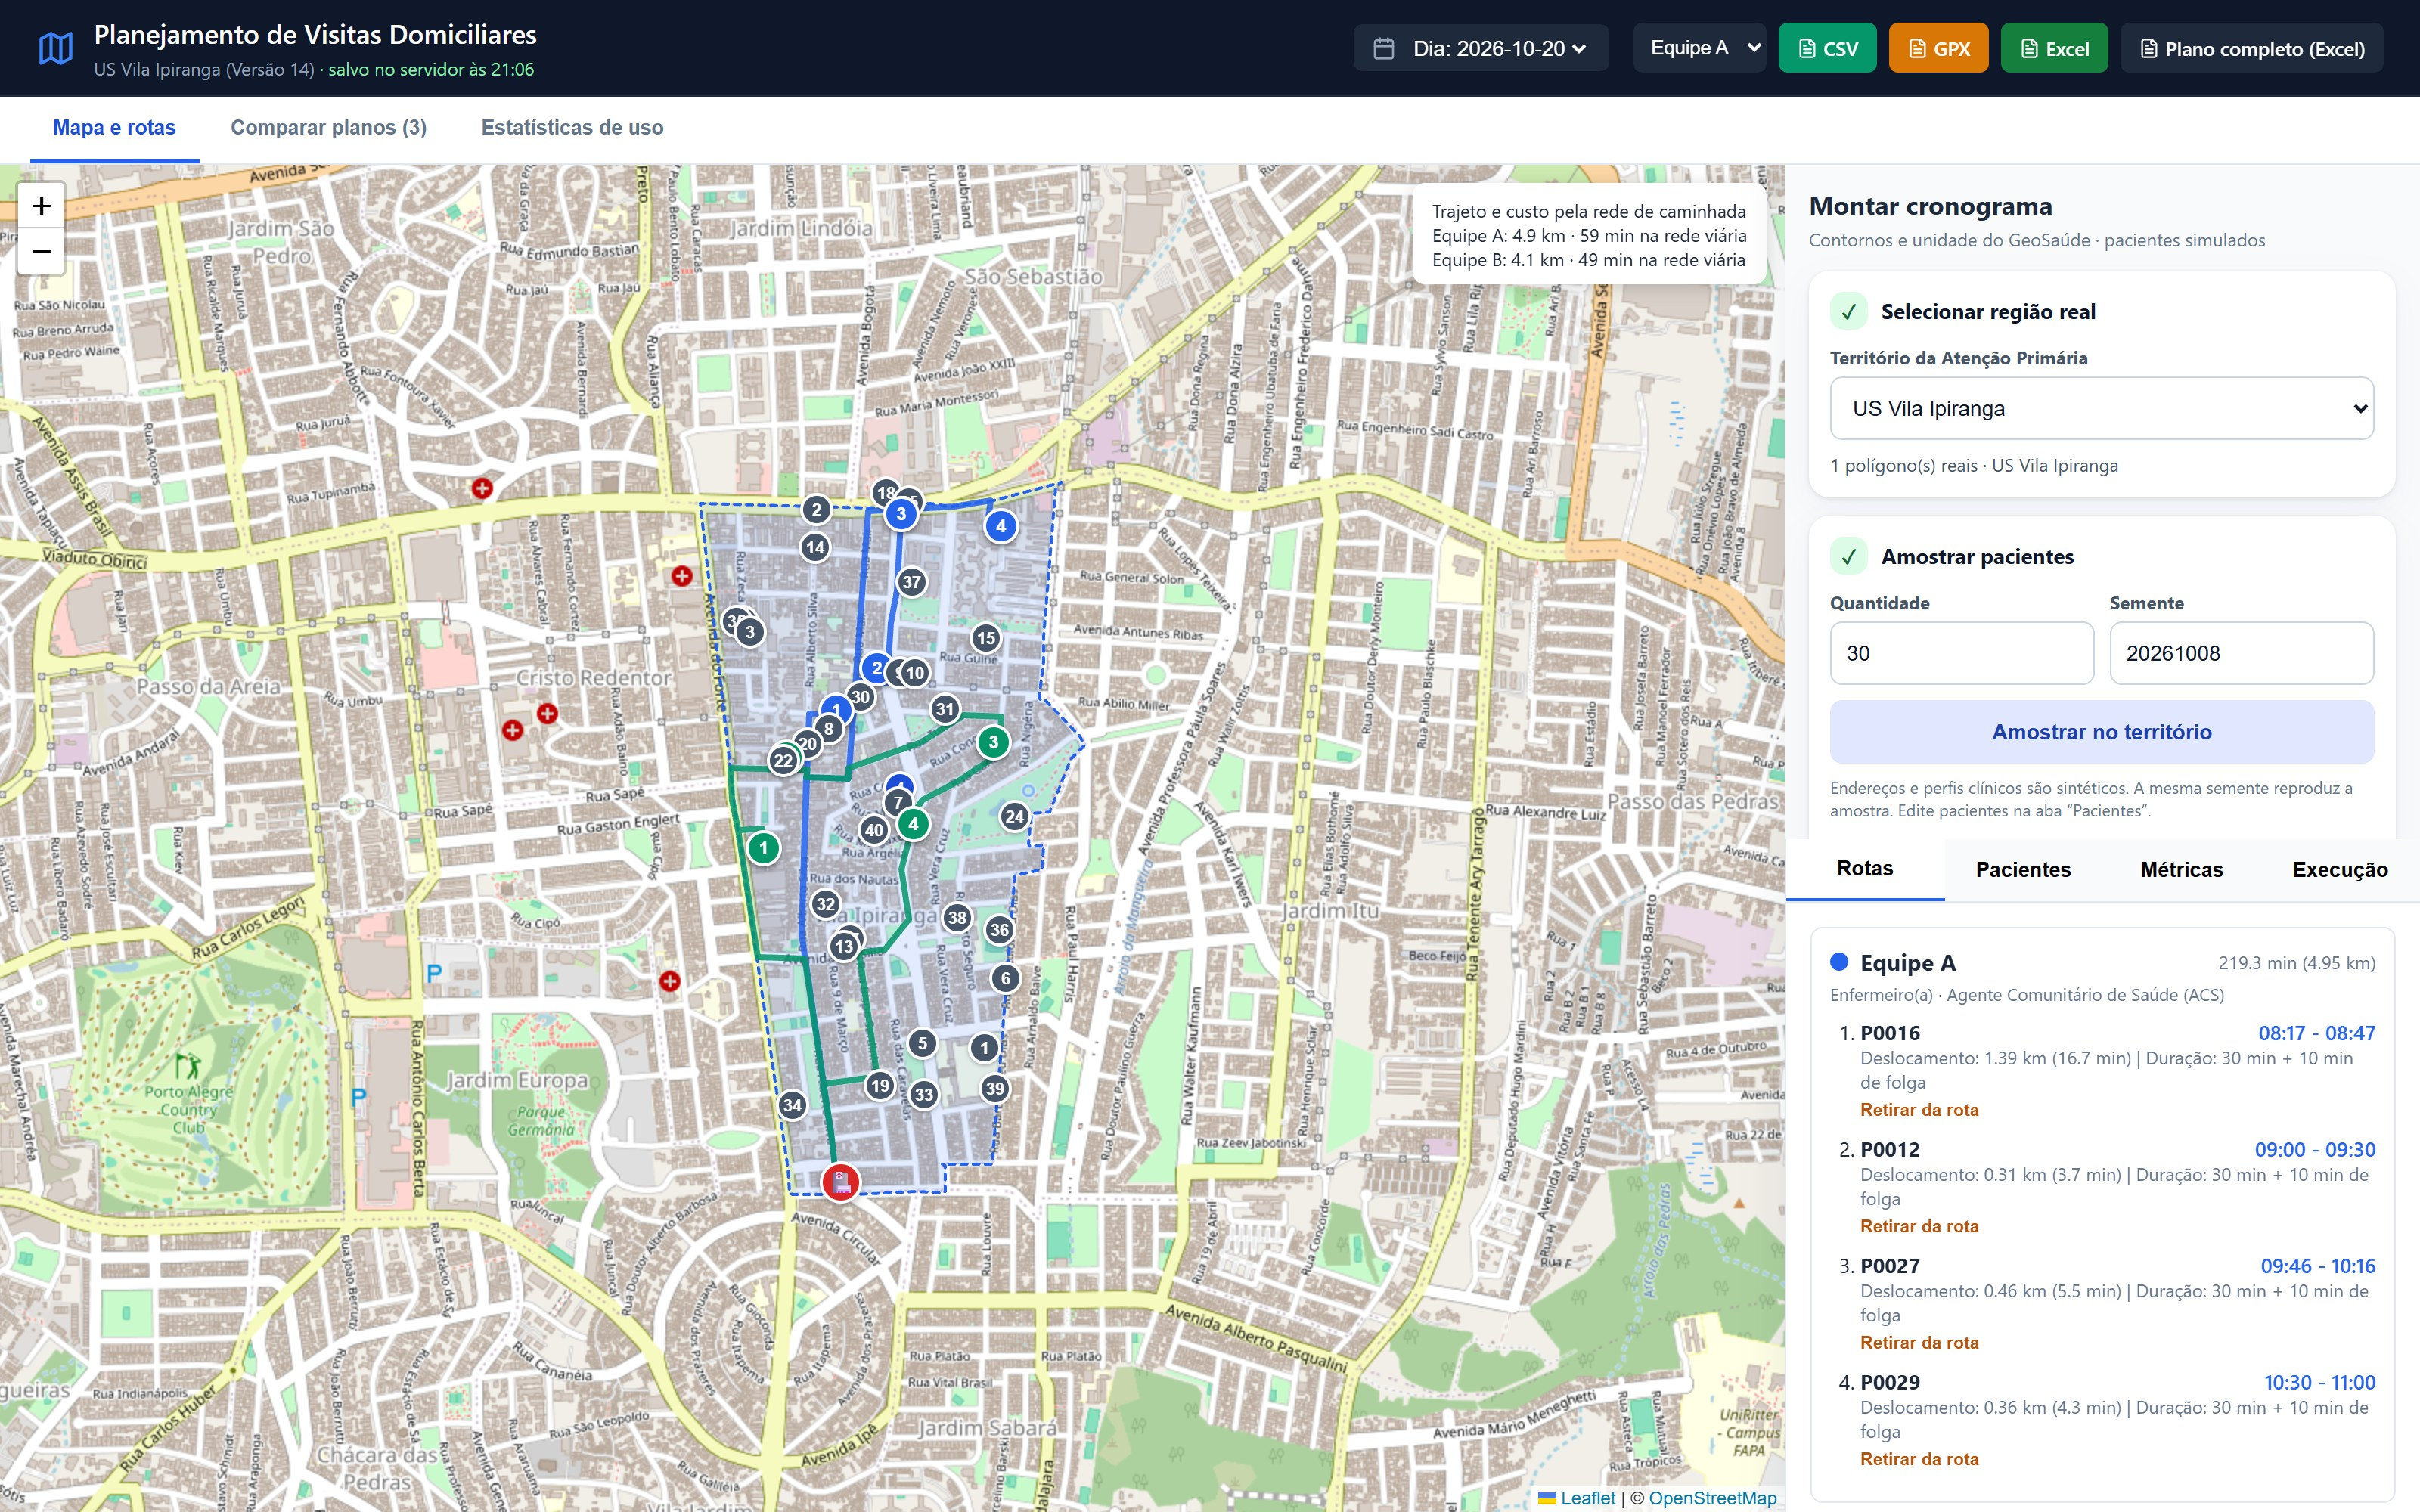
\includegraphics[width=\columnwidth]{mapa-rotas.jpg}
\caption{Interface do artefato: território GeoSaúde, rotas a pé de duas equipes num dia e a agenda da equipe A. Pacientes sintéticos.}
\label{fig:interface}
\end{figure}

\section{Desenho experimental}\label{sec:desenho}

\subsection{Questões de pesquisa}

\begin{itemize}
  \item[\textbf{QP1}] Na cidade inteira, a busca mensal atende mais prioridade a tempo que as referências, e a que custo de caminhada?
  \item[\textbf{QP2}] Como o efeito varia com o número de pacientes, a área, o horizonte, o atraso inicial e a taxa de faltas?
  \item[\textbf{QP3}] Num acúmulo grande de visitas, qual método conclui tudo antes?
  \item[\textbf{QP4}] Os planos respeitam todas as restrições, inclusive sob combinações extremas?
\end{itemize}

\subsection{Instâncias e simulação}

Os territórios e as unidades são os 132 do GeoSaúde de Porto Alegre. Os pacientes são sintéticos: localizações sorteadas dentro dos polígonos e perfis clínicos copiados de modelos, com o gerador Mulberry32 e sementes fixas. Nos experimentos, as matrizes vêm da API Table do OSRM com o perfil de caminhada, e cada instância usa a mesma matriz nas três estratégias. A falta é sorteada por paciente e data com números aleatórios comuns: o mesmo sorteio vale para as três estratégias e para os três níveis de falta (0\%, 5\% e 10\% por tentativa). A simulação executa cada dia útil, registra os resultados e refaz o plano. Instâncias sem caminho a pé completo são excluídas e listadas.

\begin{itemize}
  \item \textbf{E1, cidade} (QP1): 131 territórios com caminho completo, 30 pacientes cada, uma equipe de 240~min/dia, 22 dias úteis; $131 \times 3$ níveis de falta $= 393$ pares por comparação.
  \item \textbf{E2, fatorial} (QP2): território da US Restinga; 3 sementes $\times$ 4 quantidades de pacientes (15, 30, 45, 90) $\times$ 3 áreas (0,5$\times$, 1$\times$, 2$\times$ o polígono) $\times$ 3 horizontes (5, 10, 22 dias) $\times$ 3 proporções de visitas já vencidas (0, 25, 50\%) $= 324$ cenários; uma equipe de 240~min/dia, $A=2$; 972 pares.
  \item \textbf{E3, acúmulo} (QP3): 250 pacientes na Restinga, uma equipe de 300~min/dia, prazos entre outubro de 2026 e janeiro de 2027 e limite comum de 12 meses (261 dias úteis); 3 sementes $\times$ 3 níveis de falta; mede-se quantos dias úteis cada método leva para concluir as 250 visitas.
  \item \textbf{E4, propriedades} (QP4): 300 cenários aleatórios com restrições combinadas (âncoras, categorias e quantidades, vínculos, ausências, folgas, equipes de folga) nas três estratégias.
\end{itemize}

\subsection{Análise}

As comparações são pareadas: no mesmo cenário e com o mesmo nível de falta, compara-se a busca mensal a cada referência e contam-se vitórias, empates e derrotas. Relatamos médias e medianas descritivas. Não aplicamos testes de hipótese: os pares de um mesmo cenário compartilham pacientes e sorteios entre níveis de falta, e não são independentes.

\section{Resultados}\label{sec:resultados}

\subsection{QP1: cidade inteira}

A Tabela~\ref{tab:cidade} resume E1. A busca mensal atendeu a tempo 34,63\% dos pontos de prioridade, 6,45\pp\ acima do vizinho mais próximo (22,9\% relativos) e caminhou 1,1\% menos. Venceu 307 dos 393 pares em prioridade a tempo, empatou 58 e perdeu 28; caminhou mais em 156 pares. A cobertura total quase não muda entre os métodos: o ganho está em \emph{quando} e \emph{quem} é atendido, não em quantos. O custo é computacional: cerca de dez vezes o tempo do vizinho, ainda 0,13~s por simulação mensal.

\begin{table}[t]
\centering
\caption{E1: médias em 131 territórios $\times$ 3 níveis de falta}
\label{tab:cidade}
\footnotesize
\begin{tabular}{@{}lrrr@{}}
\toprule
Indicador & Busca mensal & Vizinho & Urgência \\
\midrule
Prioridade a tempo $\Phi$ (\%) & \textbf{34,63} & 28,18 & 17,93 \\
Cobertura efetiva (\%) & 98,07 & 98,23 & 98,55 \\
Atraso controlável (dias) & \textbf{2,76} & 3,07 & 3,69 \\
Distância a pé (km) & \textbf{69,60} & 70,40 & 97,06 \\
Cálculo acumulado (ms) & 131,87 & 12,78 & 9,00 \\
\bottomrule
\end{tabular}
\end{table}

\subsection{QP2: grade fatorial}

Frente ao vizinho mais próximo, a busca mensal ganhou em média 9,65\pp\ de prioridade a tempo (mediana 6,62\pp) e 0,55 dia de atraso controlável ponderado (Tabela~\ref{tab:fatorial}). Ao contrário de E1, caminhou 3,03\% mais em média (113,16 contra 109,83~km), e mais em 473 dos 972 pares: na grade, com mais carga por equipe, a heurística troca caminhada por prioridade. Frente à urgência, venceu todos os 972 pares em prioridade a tempo e em atraso, e caminhou 21,54~km menos em média. Os cinco piores pares vêm de dois cenários; o pior (15 pacientes, área original, 5 dias, 50\% já vencidas) perde 4,09\pp, igual nos três níveis de falta.

\begin{table}[t]
\centering
\caption{E2: ganho pareado da busca mensal (972 pares)}
\label{tab:fatorial}
\footnotesize
\setlength{\tabcolsep}{3.5pt}
\begin{tabular}{@{}llrrr@{}}
\toprule
Ref. & Métrica & Média & Mediana & V/E/D \\
\midrule
\multirow{4}{*}{Vizinho} & Prioridade a tempo (p.p.) & 9,65 & 6,62 & 899/64/9 \\
 & Atraso controlável (dias) & 0,55 & 0,39 & 943/6/23 \\
 & Distância (km) & $-$3,33 & 0,00 & 284/215/473 \\
 & Cobertura (p.p.) & 0,90 & 0,00 & 271/619/82 \\
\midrule
\multirow{4}{*}{Urgência} & Prioridade a tempo (p.p.) & 20,84 & 18,37 & 972/0/0 \\
 & Atraso controlável (dias) & 2,07 & 1,46 & 972/0/0 \\
 & Distância (km) & 21,54 & 15,30 & 813/77/82 \\
 & Cobertura (p.p.) & 12,50 & 12,78 & 635/324/13 \\
\bottomrule
\multicolumn{5}{@{}p{0.95\columnwidth}@{}}{\scriptsize Ganho positivo favorece a busca mensal; em distância, negativo significa mais caminhada. V/E/D: vitórias, empates e derrotas.}
\end{tabular}
\end{table}

O ganho frente ao vizinho cai pouco com a taxa de faltas (Fig.~\ref{fig:faltas}): de 9,91 para 9,47\pp\ em E2 e de 6,91 para 5,94\pp\ em E1, entre 0\% e 10\% de faltas por tentativa.

\begin{figure}[t]
\centering
\begin{tikzpicture}
\begin{axis}[
  width=\columnwidth, height=4.6cm,
  ybar, bar width=9pt, ymin=0, ymax=12,
  symbolic x coords={0\%,5\%,10\%}, xtick=data,
  xlabel={Faltas por tentativa}, ylabel={Ganho (p.p.)},
  ylabel style={font=\footnotesize}, xlabel style={font=\footnotesize},
  tick label style={font=\footnotesize},
  legend style={font=\footnotesize, at={(0.5,1.02)}, anchor=south, legend columns=2, draw=none},
  nodes near coords, nodes near coords style={font=\scriptsize, /pgf/number format/use comma, /pgf/number format/fixed, /pgf/number format/precision=2},
  enlarge x limits=0.25]
\addplot[fill=black!25, draw=black!60] coordinates {(0\%,6.91) (5\%,6.52) (10\%,5.94)};
\addplot[fill=blue!35, draw=blue!60!black] coordinates {(0\%,9.91) (5\%,9.57) (10\%,9.47)};
\legend{E1 (cidade), E2 (fatorial)}
\end{axis}
\end{tikzpicture}
\caption{Ganho médio de prioridade atendida a tempo frente ao vizinho mais próximo, por taxa de faltas.}
\label{fig:faltas}
\end{figure}

\subsection{QP3: acúmulo de 250 pacientes}

Com quatro meses, a busca mensal colocou 249 a 250 das 250 visitas no plano inicial, contra 241 a 243 do vizinho e 246 a 248 da urgência. Com o limite de 12 meses, as 27 execuções concluíram todas as visitas (Tabela~\ref{tab:longo}). Nos 9 pares, a busca mensal terminou em 88,11 dias úteis, contra 93,67 do vizinho ($-5,56$), e caminhou 13,03\% menos; a vantagem em dias cresce com as faltas, de 3,67 para 8,33 dias úteis. O custo computacional somado de todos os replanejamentos de uma execução foi de 22 a 179~s (de 5 a 22~s por replanejamento, com horizonte de até 261 dias úteis), contra menos de 0,2~s das referências.

\begin{table}[t]
\centering
\caption{E3: dias úteis até concluir 250 visitas e caminhada (médias de 3 sementes)}
\label{tab:longo}
\footnotesize
\setlength{\tabcolsep}{4pt}
\begin{tabular}{@{}lrrrrrr@{}}
\toprule
& \multicolumn{2}{c}{Busca mensal} & \multicolumn{2}{c}{Vizinho} & \multicolumn{2}{c}{Urgência} \\
\cmidrule(lr){2-3}\cmidrule(lr){4-5}\cmidrule(l){6-7}
Faltas & dias & km & dias & km & dias & km \\
\midrule
0\% & \textbf{87,67} & \textbf{1.103} & 91,33 & 1.273 & 88,33 & 1.342 \\
5\% & \textbf{88,33} & \textbf{1.123} & 93,00 & 1.291 & 89,33 & 1.419 \\
10\% & \textbf{88,33} & \textbf{1.179} & 96,67 & 1.352 & 91,67 & 1.460 \\
\bottomrule
\end{tabular}
\end{table}

\subsection{QP4: propriedades dos planos}

Os 900 planos de E4 foram aceitos pelo verificador, sem duplicatas, com equipes compatíveis, horários ordenados, totais de rota iguais aos da matriz e jornadas respeitadas; todo prazo rígido foi agendado a tempo ou ficou pendente como obrigatório, com motivo. Para estimar a sensibilidade dos testes, desativamos, uma de cada vez, a regra de ausência e a de quantidade por categoria no código compilado: as suítes falharam nos dois casos. Ao todo, o núcleo tem 47 testes automáticos (métricas, busca mensal, amostragem, restrições, limites, operações de campo e importação) e o servidor, 3. Por fim, sem as restrições novas, reexecutar E1--E3 com as matrizes em cache reproduziu as 5.103 linhas de resultados sem nenhuma diferença.

\section{Discussão}

Os resultados apoiam a hipótese quanto à prioridade e ao atraso: nos três estudos, a busca mensal atende mais pontos de prioridade a tempo e acumula menos atraso controlável que as duas referências. Quanto ao deslocamento, o apoio é parcial. Na cidade e no acúmulo, ela caminha menos que o vizinho; na grade fatorial, caminha 3\% mais. Os movimentos da busca nunca aumentam a caminhada além do orçamento da fase, mas a segunda fase reinsere pendências antes de fixar esse orçamento: a busca atende mais visitas (cobertura 0,90\pp\ maior em E2), e essas visitas custam caminhada.

A regra de urgência mostra o risco de priorizar sem olhar o mapa: atende os mais urgentes primeiro, mas cruza o território e esgota a jornada, perdendo em prioridade a tempo e em distância. O vizinho economiza caminhada mas ignora prazos. A busca mensal combina os dois ao mover visitas entre dias, o que nenhuma das referências faz.

O custo computacional é o principal preço: cerca de 0,13~s por mês simulado em E1, e menos de 1~s por plano mensal em toda a grade fatorial, com até 90 pacientes. Num acúmulo de 250 pacientes com horizonte de 261 dias úteis, porém, cada replanejamento levou de 5 a 22~s, e os replanejamentos de uma execução somaram até 179~s; horizontes longos pedem uma busca incremental.

\section{Ameaças à validade}

\textbf{Construto.} $\Phi$ depende dos pesos clínicos, aqui sintéticos; outros pesos podem mudar a ordem dos métodos. Medimos eficiência do plano, não benefício clínico.

\textbf{Interna.} $\lambda$ e $\mu$ foram fixados por julgamento, não ajustados; a comparação usa os mesmos sorteios, matrizes e demanda, o que reduz confusão entre métodos.

\textbf{Externa.} Pacientes, prazos e faltas são sintéticos, com uma amostra por território em E1. E2 e E3 usam um único território, e o mapa usado nesses estudos não cobria bem a Restinga: as comparações entre métodos se mantêm, mas os quilômetros absolutos daquele território devem ser recalculados com o mapa atual. A falta foi modelada como sorteio independente por tentativa.

\textbf{Conclusão.} Os números são descritivos de três sementes e níveis escolhidos, sem intervalos de confiança.

\section{Conclusão}

Formulamos o planejamento mensal de visitas domiciliares a pé na APS com restrições levantadas junto a agentes de saúde e propusemos uma busca local mensal que, em três estudos sobre territórios reais de Porto Alegre, atendeu mais prioridade clínica a tempo e acumulou menos atraso que regras simples, com caminhada igual ou menor em dois dos três estudos. O artefato roda sem infraestrutura externa e verifica formalmente cada plano. Os próximos passos são um estudo com agentes de uma unidade usando o cadastro real, a repetição de E2 e E3 com o mapa atual e o roteador interno, a calibração de $\lambda$ e $\mu$ com as equipes e uma garantia de prazos rígidos que reorganize âncoras já colocadas.

\section*{Disponibilidade}

Código, cenários, resultados e diário de bordo: \url{https://github.com/vitorsfeijo/inf99003-project_2-group_A}.

\section*{Agradecimentos}

Aos agentes de saúde ouvidos em 06/11/2026 e a Fabio Cieslak, Tobias Marion e Vitor Feijo, que construíram a primeira versão do artefato no ciclo anterior da disciplina INF99003.

\bibliographystyle{IEEEtran}
\bibliography{../referencias}

\end{document}
